\section{Recording provenance of workflow runs with RO-Crate}
\label{ch54:wrroc}

Recording the provenance of scientific computation results is key to the support of traceability, reproducibility and quality assessment of data products.
Several data models have been explored to address this need, providing representations of workflow plans and their executions as well as means of packaging the resulting information for archiving and sharing.
However, existing approaches tend to lack interoperable adoption across workflow management systems.

In this work we present \textbf{Workflow Run RO-Crate}, an extension of RO-Crate (Research Object Crate) and Schema.org to capture the provenance of the execution of computational workflows at different levels of granularity and bundle together all their associated products (inputs, outputs, code, etc.).
The model is supported by a diverse, open community that runs regular meetings, discussing development, maintenance and adoption aspects.
Workflow Run RO-Crate is already implemented by several workflow management systems, allowing interoperable comparisons between workflow runs from heterogeneous systems.
We describe the model, its alignment to standards such as W3C PROV, and its implementation in six workflow systems.
Finally, we illustrate the application of Workflow Run RO-Crate in two use cases of machine learning in the digital image analysis domain.



\subsection{Introduction}\label{ch54:introduction}

A crucial part of scientific research is recording the provenance of its outputs.
The W3C PROV standard defines provenance as ``a record that describes the people, institutions, entities, and activities involved in producing, influencing, or delivering a piece of data or a thing''
\cite{Moreau 2013}.
Provenance is instrumental to activities such as traceability, reproducibility, accountability, and quality assessment
\cite{Herschel 2017}.
The constantly growing size and complexity of scientific datasets and the analysis that is required to extract useful information from them has made science increasingly dependent on advanced automated processing techniques in order to get from experimental data to final results~\cite{Himanen 2019, Gauthier 2019, Huntingford 2019}.
Consequently, a large part of the provenance information for scientific outputs consists of descriptions of complex computer-aided data processing steps. This data processing is often expressed as workflows, i.e., high-level applications that coordinate multiple tools and manage intermediate outputs in order to produce the final results.

In order to homogenise the collection and interchange of provenance records, the W3C consortium proposed the PROV-O standard~\cite{w3-prov-o}, an OWL \cite{w3-owl2-overview} representation of PROV for provenance in the Web.
PROV-O has been widely extended for workflows (D-PROV \cite{Missier 2013}, ProvONE \cite{Cuevas-Vicenttín 2016}, OPMW \cite{Garijo 2011}, P-PLAN \cite{Garijo 2012}), where provenance information is collected in two main forms: prospective and retrospective~\cite{Freire 2008}. \emph{Prospective provenance} -- the execution plan -- is essentially the workflow itself: it includes a machine-readable specification with the processing steps to be performed and the data and software dependencies to carry out each computation.
\emph{Retrospective provenance} refers to what actually happened during an execution, i.e.~what were the values of the input parameters, which outputs were produced, which tools were executed, how much time did the execution take, whether the execution was successful or not, etc.
Retrospective provenance can also be represented at different levels of abstraction depending on available computing resources: for instance, by the workflow execution becoming a single activity which produces results, by specifying the individual execution of each workflow step, or by going a step further and indicating how each step is divided into sub-processes when a workflow is deployed in a cluster.

Different workflow systems have adopted and extended PROV (and its PROV-O representation) to the workflow domain (WINGS \cite{Gil 2011, Garijo 2014}, VisTrails \cite{Scheidegger 2008,Costa 2013}), in order to ease the burden of provenance collection from tool developers to workflow management systems (WMS) \cite{Atkinson 2017,Pérez 2018}.

D-PROV, PROV-ONE, OPMW-PROV, P-Plan propose representations of workflow plans and their respective executions, taking into account the features of the workflow systems implementing them (e.g., hierarchical representations, sub-processes, etc.).
Other data models like \emph{wfprov} and \emph{wfdesc}
\cite{Belhajjame 2015} go a step further by considering not only the link between plans and executions, but how to package the various artefacts as a Research Object (RO) ~\cite{Bechhofer 2013} in order to ease portability while keeping the context of a digital experiment.

However, while these models address some workflow provenance representation issues, they have two main limitations: Firstly, the extensions of PROV are not directly interoperable because of differences in granularity or different assumptions in their workflow representations; secondly, their support from WMS is typically one system per model.  An early approach to unify and integrate workflow provenance traces across WMS was WEST (Workflow Ecosystems through STandards) \cite{Garijo 2014}, through the use of WINGS \cite{Gil 2011} to build workflow templates and different converters. 

In all of these workflow provenance models, the emphasis is on the workflow execution structure as a directed graph, with only partial references for the data items. 
The REPRODUCE-ME ontology \cite{Samuel 2022} extended PROV and P-Plan to explain the overall scientific process with the experimental context including real life objects (e.g. instruments, specimens) and human activities (e.g. lab protocols, screening), demonstrating provenance of individual Jupyter Notebook \footurl{https://sheeba-samuel.github.io/REPRODUCE-ME/research/provbook.html}{cells} and highlighting the need for provenance also where there is no workflow management system. 

More recently, interoperability have been partially addressed by Common Worlflow Language Prov (CWLProv)~\cite{Khan 2019}, which represents workflow enactments as ROs serialised according to the Big Data Bag (BDBag) approach~\cite{Chard 2016}.
The resulting format is a folder containing several data and metadata files~\cite{Soiland-Reyes 2018}, expanding on the RO Bundle approach of Taverna \cite{Soiland-Reyes 2016}.
CWLProv also extends PROV with a representation of executed processes (activities), their inputs and outputs (entities) and their executors (agents), together with their Common Workflow Language specification
\cite{Crusoe 2022} -- a standard workflow specification adopted by at least a dozen different  \footurl{https://www.commonwl.org/implementations/}{workflow systems}. Although CWLProv includes prospective provenance as a \emph{plan}
within PROV (based on the \emph{wfdesc} model), in practice its implementation does not include tool definitions or file formats, as proposed by the wfdesc extension \footurl{https://wf4ever.github.io/ro/2016-01-28/roterms}{Roterms}.
In order for CWLProv consumers to reconstruct the full prospective provenance for understanding the workflow, they would also need to inspect the separate workflow definition in the native language of the WMS.
Additionally, the CWLProv RO may include several other metadata files and PROV serialisations conforming to different formats, complicating its generation and consumption.

As for granularity, CWLProv proposed multiple levels of provenance \cite[figure 2]{Khan 2019}, from Level 0 (capturing workflow definition) to Level 3 (domain-specific annotations). 
In practice, the CWL reference implementation \emph{cwltool} \cite{Amstutz 2023} and the corresponding CWLProv specification \cite{Soiland-Reyes 2018} records provenance details of all task executions together with the intermediate data and any nested workflows (CWLProv level 2), a granularity level that requires substantial support from the WMS.
This approach is appropriate for workflow languages where the execution plan, including its distribution among the various tasks, is well known in advance (such as CWL).
However, it can be at odds with other systems where the execution is more dynamic, depending on the verification of specific runtime conditions, such as the size and distribution of the data (e.g., COMPSs~\cite{Lordan 2014}).

This makes the implementation of CWLProv challenging, as shown by the fact that at the time of writing the format is supported only by cwltool.
Finally, being based on the PROV model, CWLProv is highly focused on the interaction between agents, processes and related entities, while support for contextual metadata (such as workflow authors, licence or creation date) in the Research Object Bundle is \footurl{https://w3id.org/bundle/context}{limited} and stored in a separate manifest file, that includes the data identifier mapping to filenames.
A project that uses serialised ROs similar to those used by CWLProv is Whole Tale \cite{Chard 2019}, a web platform with a focus on the narrative around scientific studies and their reproducibility, where the serialised ROs are used to export data and metadata from the platform. In contrast, our work is primarily focused on the ability to capture the provenance of computational workflow execution including its data and executable workflow definitions.

RO-Crate~\cite{Soiland-Reyes 2022} is a recent approach to packaging research data together with their metadata; it extends Schema.org~\cite{Guha 2015}, a popular vocabulary for describing resources on the Web.
In its simplest form, an RO-Crate is a directory structure that contains a single JSON-LD \cite{w3-json-ld} metadata file at the top level.
The metadata file describes all entities stored in the RO-Crate along with their relationships; it is both machine-readable and human-readable.
RO-Crate is general enough to be able to describe any dataset, but can also be made as specific as needed through the use of extensions called
\emph{profiles}.
At the same time, the broad set of types and properties from Schema.org, complemented by a few additional terms from other vocabularies, make the RO-Crate model capable of expressing a wide range of contextual information that complements and enriches the core information specified by the profile.
This may include, among others, the workflow authors and their affiliations, associated publications, licensing information, related software, etc.
This is an approach used by WorkflowHub \cite{Goble 2021}, a workflow system agnostic workflow registry which specifies a Workflow RO-Crate profile \cite{Bacall 2022} to gather the workflow definition with such metadata in an archived RO-Crate. 

In this work, we present \textbf{Workflow Run RO-Crate} (WRROC), an extension of RO-Crate for representing computational workflow execution provenance.
Our main contributions are the following:

\begin{itemize}
\item   A collection of RO-Crate profiles to represent and package both the prospective and the retrospective provenance of a computational workflow run in a way that is machine-actionable \cite{Batista 2022},  independent of the specific workflow language or execution system, and including support for reexecution.
\item   Implementations of the model in six workflow management systems and one conversion tool.
\item   A mapping of our profiles against the W3C PROV-O Standard using the Simple Knowledge Organisation System (SKOS) \cite{w3-skos-primer}.
\end{itemize}

To foster usability, the profiles are characterised by different levels of detail, and the set of mandatory metadata items is kept to a minimum in order to ease the implementation.
This flexible approach increases the model's adaptability to the diverse landscape of WMS used in practice.
The base profile, in particular, is applicable to any kind of computational process, not necessarily described in a formal workflow language.
All profiles are supported and sustained by the Workflow Run RO-Crate community, which meets regularly to discuss extensions, issues and new implementations.

The rest of this work is organised as follows: we first describe the Workflow Run RO-Crate profiles; we then illustrate implementations and usage examples; this is followed by a discussion and plans for future work.


%% 
\subsection{The Workflow Run RO-Crate profiles}\label{ch54:the-workflow-run-ro-crate-profiles}

RO-Crate profiles are extensions of the base RO-Crate specification that describe how to represent the entities and relationships that appear in a specific domain or use case.
An RO-Crate conforming to a profile is not just machine-readable, but also machine-actionable as a digital object whose type is represented by the profile itself~\cite{10.3897/rio.8.e93937}.

The Workflow Run RO-Crate profiles are the main outcome of the activities of the Workflow Run RO-Crate \footurl{https://www.researchobject.org/workflow-run-crate}{Community}, an open working group that includes workflow users and developers, WMS users and developers, and researchers and software engineers interested in workflow execution provenance and Findable, Accessible, Interoperable and Reusable (FAIR) approaches for data and software.
In order to develop the Workflow-Run RO-Crate profiles, one of the first community efforts was to compile a list of requirements in the form of competency \footurl{https://www.researchobject.org/workflow-run-crate/requirements}{questions} to be addressed by the model.
Each requirement was backed up by a rationale and linked to a GitHub issue to drive the public discussion forward. When a requirement was addressed, related changes were integrated into the profiles and the relevant issue was closed. Many of the original issues are now closed, and the profiles have had four official releases on Zenodo.


As requirements were being defined, it became apparent that one single profile would not have been sufficient to cater for all possible usage scenarios.
In particular, while some use cases required a detailed description of all computations orchestrated by the workflow, others were only concerned with a ``black box'' representation of the workflow and its execution as a whole (i.e., whether the execution was successful and which results were obtained).
Additionally, some computations involve a data flow across multiple applications that are executed without the aid of a WMS and thus are not formally described in a standard workflow language.
These observations led to the development of three profiles: 

\begin{enumerate}[(1)]
  \item \footurl{https://w3id.org/ro/wfrun/process}{Process Run Crate}
  to describe the execution of one or more tools that contribute to a computation.
  \item \footurl{https://w3id.org/ro/wfrun/workflow}{Workflow Run Crate}
  to describe a computation orchestrated by a predefined workflow.
  \item \footurl{https://w3id.org/ro/wfrun/provenance}{Provenance Run Crate}
  to describe a workflow computation including the internal details of individual step executions.
\end{enumerate}

In the rest of this section we describe each of the above profiles in detail.
We use italics to denote the types and properties describing entities and their relationships: these are defined in the RO-Crate JSON-LD \footurl{https://www.researchobject.org/ro-crate/1.1/context.jsonld}{context}, which extends Schema.org with terms from the Bioschemas \cite{Gray 2017} ComputationalWorkflow \footurl{https://bioschemas.org/profiles/ComputationalWorkflow/1.0-RELEASE}{profile} and other vocabularies. More specifically, from Bioschemas we use the \emph{ComputationalWorkflow} and \emph{FormalParameter} types as well as the \emph{input} and \emph{output} properties. 
Note that these terms, though coming from Bioschemas, are not specific to the life sciences.
We also developed a context extension through a dedicated ``workflow-run'' \footurl{https://w3id.org/ro/terms/workflow-run\#}{namespace} to represent concepts that are not captured by terms in the RO-Crate context.

\subsubsection{Process Run Crate}\label{ch54:process-run-crate}

The Process Run Crate profile \cite{WRROC 2023a} contains specifications on describing the execution of one or more software applications that contribute to the same overall computation, but are not necessarily coordinated by a top-level workflow or script.
For instance, they could be executed manually by a human agent, one after the other as intermediate datasets become available, as shown in the process run \footurl{https://w3id.org/ro/doi/10.5281/zenodo.6913045}{crate} from \cite{Meurisse 2023}.

Being the basis for all profiles in the WRROC collection, Process Run Crate specifies how to describe the fundamental entities involved in a computational run: a software application (represented by a
\emph{SoftwareApplication}, \emph{SoftwareSourceCode} or
\emph{ComputationalWorkflow} entity) and its execution (represented by a \emph{CreateAction} entity), with the latter linking to the former via the \emph{instrument} property.
Other important properties of the
\emph{CreateAction} entity are \emph{object}, which links to the action's inputs, and \emph{result}, which links to its outputs.
The time the execution started and ended can be provided, respectively, via the
\emph{startTime} and \emph{endTime} properties.
The \emph{Person} or
\emph{Organization} entity that performed the action is referred to via the \emph{agent} property.
Figure~\vref{ch54:fig:process_crate_er} shows the entities used in Process Run Crate together with their relationships.

\begin{figure}[htp]
%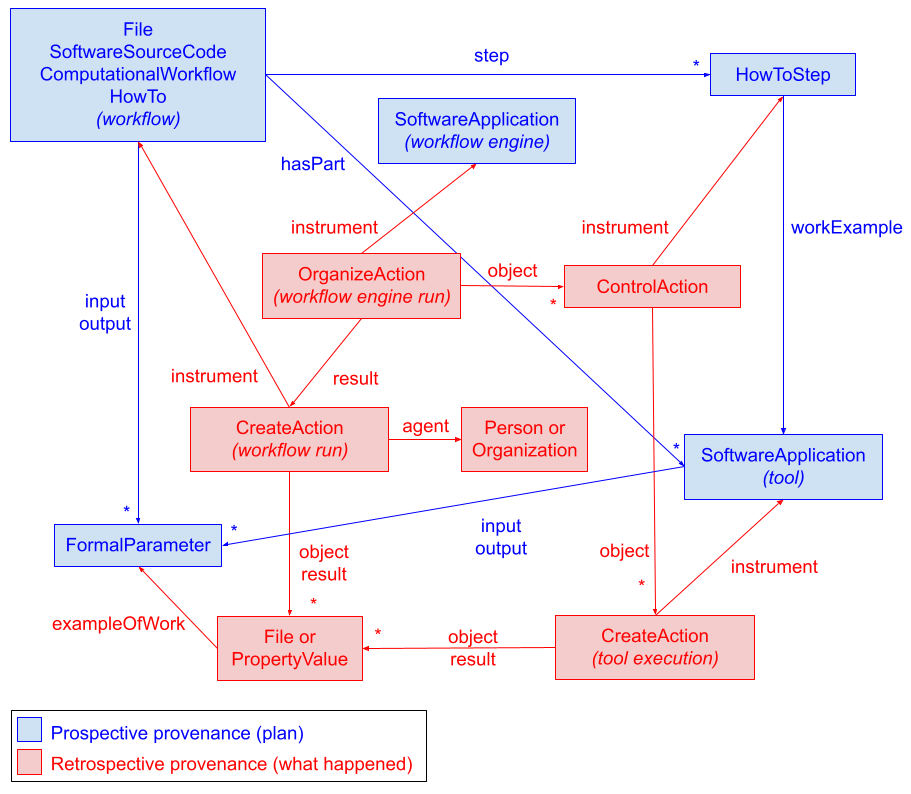
\includegraphics[width=\textwidth]{image1.png}
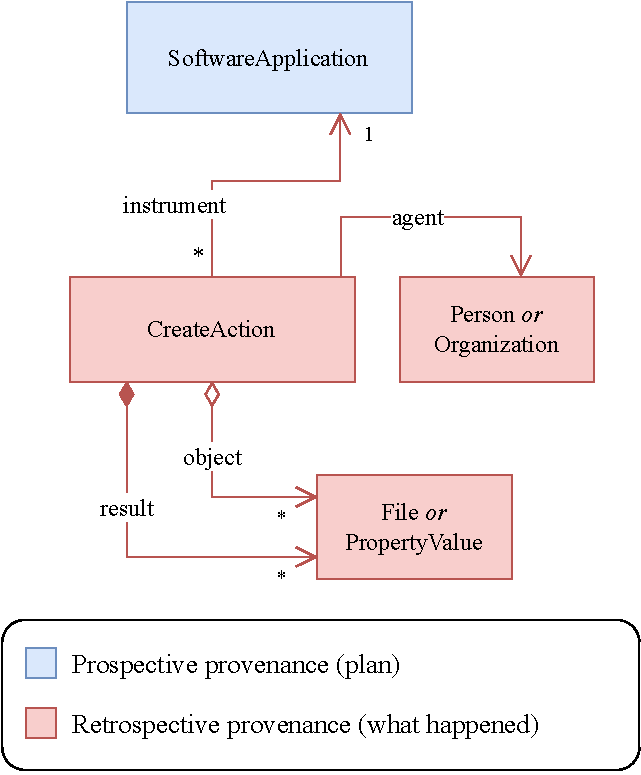
\includegraphics[width=26em]{figures/ch54/wrroc-figure1.drawio.pdf}
%\includegraphics[width=26em]{process_crate_er.eps}
\caption[UML class diagram for Process Run Crate]{{\bf UML class diagram for Process Run Crate.}
The central entity is the \emph{CreateAction}, which represents the execution of an application.
It relates with the application itself via \emph{instrument}, with the entity that executed it via \emph{agent} and with its inputs and outputs via \emph{object}
and \emph{result}, respectively. 
\emph{File} is an RO-Crate alias for Schema.org's \emph{MediaObject}.
Some inputs (and, less commonly, outputs), however, are not stored as files or directories, but passed to the application (e.g., via a command line interface) as values of various types (e.g., a number or string). In this case, the profile recommends a representation via \emph{PropertyValue}. 
For simplicity, we left out the rest of the RO-Crate structure (e.g. the root \emph{Dataset}). In this UML class notation diamond $\Diamond$ arrows indicate aggregation and regular arrows indicate references, $*$ indicates multiple instances, $1$ means single instance.  
}
\label{ch54:fig:process_crate_er}
\end{figure}

As an example,
suppose a user called John Doe runs the \texttt{head} UNIX command to extract the first ten lines of an input file named \texttt{lines.txt}, storing the result in another file called \texttt{selection.txt}.
John then runs the \texttt{sort}
command on \texttt{selection.txt}, storing the sorted output in a new file named \texttt{sorted\_selection.txt}.
Figure~\vref{ch54:fig:head_sort} contains a diagram of the two actions and their relationships to the other entities involved.
Note how the actions are connected by the fact that the output of ``Run Head'' is also the input of ``Run Sort'': they form an ``implicit workflow'', whose steps have been executed manually rather than by a software tool.

\begin{figure}[htp]
%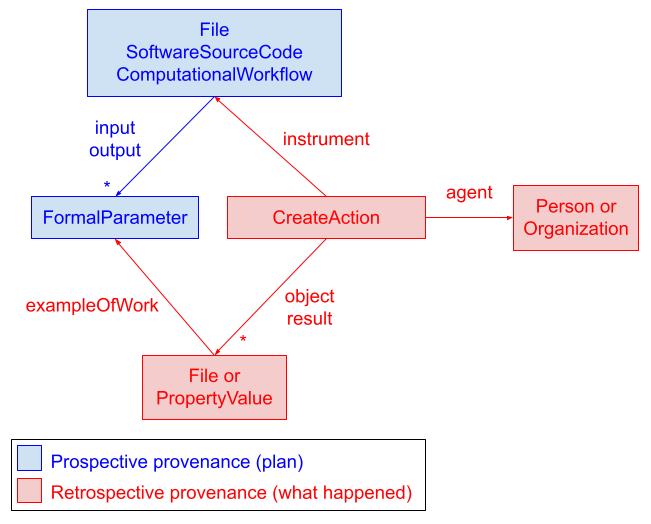
\includegraphics[width=29em]{image2.png}
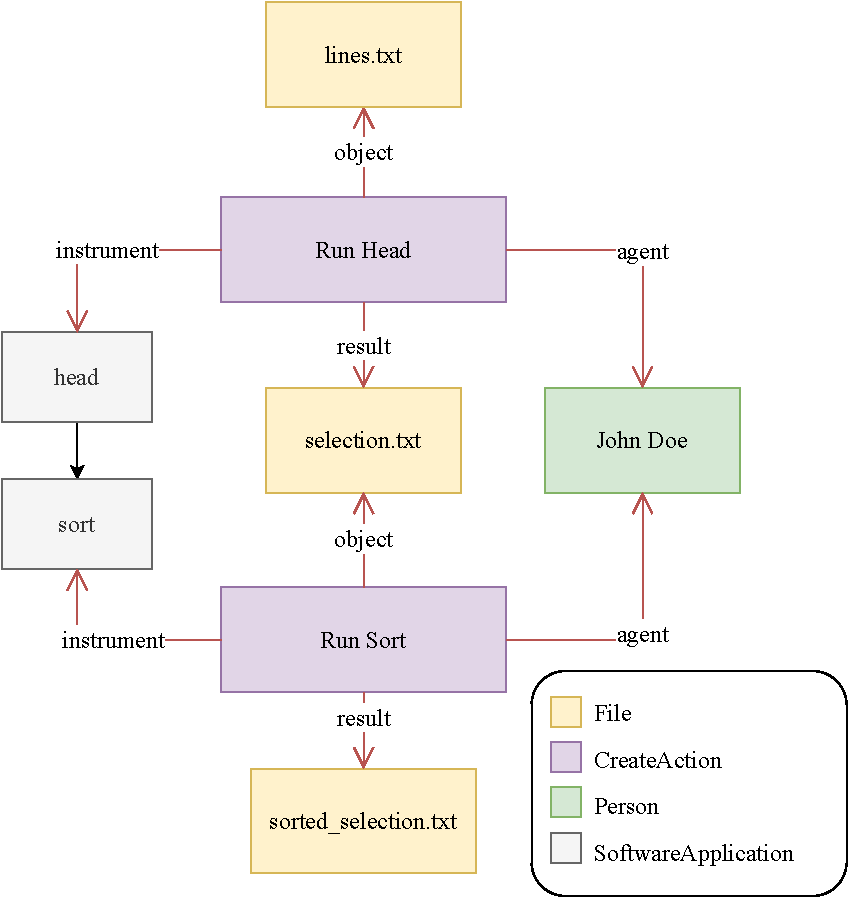
\includegraphics[width=29em]{figures/ch54/wrroc-figure-example.drawio.pdf}
%\includegraphics[width=29em]{head_sort.eps}
\caption[Diagram of a simple workflow]{{\bf Diagram of a simple workflow} where the \texttt{head} and \texttt{sort} programs were run manually by a user.
The executions of the individual software programs are connected by the fact that the file output by \texttt{head} was used as input for \texttt{sort}, documenting the computational flow in an implicit way.
Such executions can be represented with Process Run Crate.}
\label{ch54:fig:head_sort}
\end{figure}


Process Run Crate extends the RO-Crate guidelines on representing software used to create files with additional requirements and conventions.
This arrangement is typical of the RO-Crate approach, where the base specification provides general recommendations to allow for high flexibility, while profiles -- being more concerned with the representation of specific domains and machine actionability -- provide more detailed and structured definitions.
Nevertheless, in order to be broadly applicable, profiles also need to avoid the specification of too many strict requirements, trying to strike a good trade-off between flexibility and actionability.
One of the implications of this approach is that consumers need to code defensively, avoiding unwarranted assumptions -- e.g. by verifying that a value exists for an optional property before trying to retrieve it and use it.


\subsubsection{Workflow Run Crate}\label{ch54:workflow-run-crate}

The Workflow Run Crate profile \cite{WRROC 2023b} combines the Process Run Crate and WorkflowHub's Workflow RO-Crate \cite{Bacall 2022} profiles to describe the execution of “proper” computational workflows managed by a WMS.
Such workflows are typically written in a special-purpose language, such as CWL or Snakemake
\cite{Koster 2012}, and run by one or more WMS (e.g., StreamFlow \cite{Colonnelli 2021}, Galaxy~\cite{Galaxy 2022}).
As in Process Run Crate, the execution is described by a \emph{CreateAction}
that links to the application via \emph{instrument}, but in this case the application must be a workflow, as prescribed by Workflow RO-Crate.
More specifically, Workflow RO-Crate states that the RO-Crate must contain a main workflow typed as \emph{File}, \emph{SoftwareSourceCode}
and \emph{ComputationalWorkflow}.
The execution of the individual workflow steps, instead, is not represented: that is left to the more detailed Provenance Run Crate profile (described in the next section \vref{ch54:provenance-run-crate}).

The Workflow Run RO-Crate profile also contains recommendations on how to represent the workflow's input and output parameters, based on the aforementioned Bioschemas~\cite{Gray 2017} ComputationalWorkflow profile.
All these elements are represented via the \emph{FormalParameter} entity and are referenced from the main workflow via the \emph{input} and
\emph{output} properties.
While the entities referenced from
\emph{object} and \emph{result} in the \emph{CreateAction} represent data entities and argument values that were actually used in the workflow execution, the ones referenced from \emph{input} and
\emph{output} correspond to formal parameters, which acquire a value when the workflow is run (see Figure~\vref{ch54:fig:workflow_crate_er}).
In the profile, the relationship between an actual value and the corresponding formal parameter is expressed through the \emph{exampleOfWork} property -- the downloadable file is a realisation of the formal parameter definition.
For instance, in the JSON-LD snippet of Listing \vref{ch54:formalparameter} a formal parameter (\texttt{\#annotations}) is illustrated together with a corresponding \texttt{final-annotations.tsv} file:

\begin{listing}
\begin{verbatim}
{
    "@id": "#annotations",
    "@type": "FormalParameter",
    "additionalType": "File",
    "encodingFormat": "text/tab-separated-values",
    "valueRequired": "True",
    "name": "annotations"
},
{
    "@id": "final-annotations.tsv",
    "@type": "File",
    "contentSize": "14784",
    "exampleOfWork": {"@id": "#annotations"}
}
\end{verbatim}
\caption[Relating an actual value to its formal parameter definition]{{\bf Relating an actual value to its formal parameter definition.} The Bioschemas \href{https://bioschemas.org/profiles/FormalParameter/1.0-RELEASE}{\emph{FormalParameter}}\footnotemark\  entity \texttt{\#annotations} defines possible values for a workflow paramater named \texttt{annotations}. \texttt{\#final-annotations.tsv}, a downloadable \emph{File}, is an \texttt{exampleOfWork} in the sense that it realises the parameter definition.  It is also possible to flag particular values as representative exemplar values with the reverse \texttt{workExample} property from the \emph{FormalParameter}, which is not the case here. }
\label{ch54:formalparameter}
\end{listing}
\footnotetext{\url{https://bioschemas.org/profiles/FormalParameter/1.0-RELEASE}}

The derivation of Workflow Run Crate from Workflow RO-Crate makes RO-Crates that conform to this profile compatible with the WorkflowHub workflow registry by also conforming to its Workflow RO-Crate profile.
Thus, users of a WMS that implements this profile (or Provenance Run Crate, which inherits it) are able to register their workflows in WorkflowHub -- together with an execution trace -- by simply running them and uploading the resulting RO-Crates.
Additionally, the inheritance mechanism allows to reuse the specifications already developed for Workflow RO-Crate, which form part of the guidelines on representing the prospective provenance.

Figure~\vref{ch54:fig:workflow_crate_er} shows the entities used in Workflow Run Crate together with their relationships.

\begin{figure}[htp]
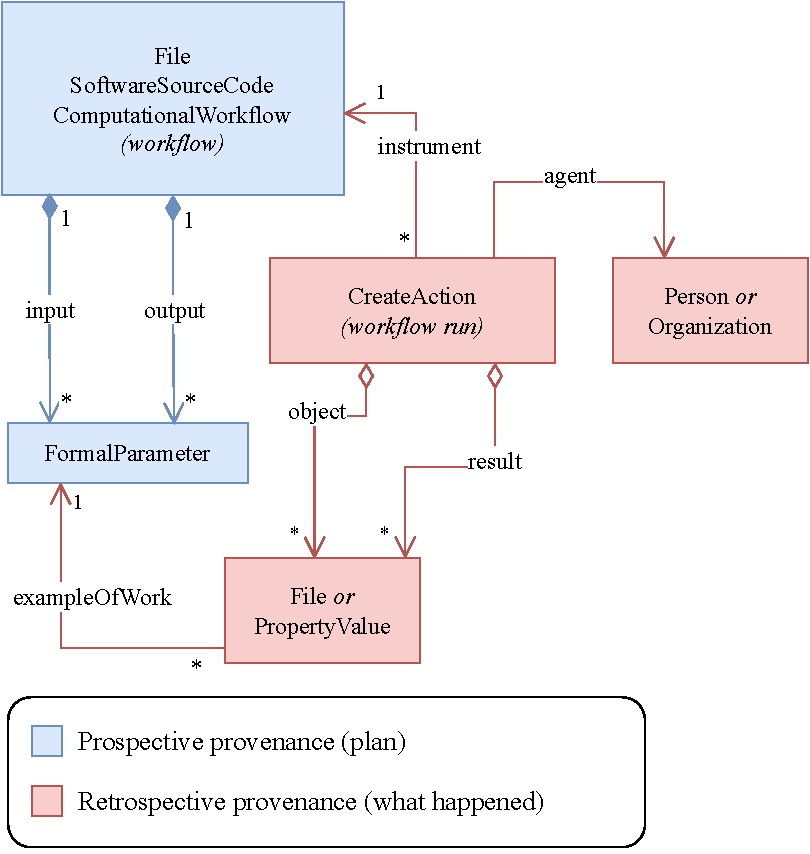
\includegraphics[width=26em]{figures/ch54/wrroc-figure2.drawio.pdf}
%\includegraphics[width=26em]{workflow_crate_er.eps}
\caption[UML class diagram]{{\bf UML class diagram for Workflow Run Crate.}
The main differences with Process Run Crate are the representation of formal parameters and the fact that the application is expected to be an entity with types \emph{File}, \emph{SoftwareSourceCode} and \emph{ComputationalWorkflow}.
Effectively, the entity belongs to all three types, and its properties are the union of the properties of the individual types.
The filled diamond $\blacklozenge$ indicates composition, empty diamond $\Diamond$ aggregation, and other arrows relations.
}
\label{ch54:fig:workflow_crate_er}
\end{figure}


\subsubsection{Provenance Run Crate}\label{ch54:provenance-run-crate}

The Provenance Run Crate profile \cite{WRROC 2023c} extends Workflow Run Crate by adding new concepts to describe the internal details of a workflow run, including individual tool executions, intermediate outputs and related parameters.
Individual tool executions are represented by additional \emph{CreateAction} instances that refer to the tool itself via \emph{instrument} -- analogously to its use in Process Run Crate.
The workflow is required to refer to the tools it orchestrates through the \emph{hasPart} property, as suggested in the Bioschemas ComputationalWorkflow profile, though in the latter it is only a recommendation.

To represent the logical steps defined by the workflow, this profile uses \footurl{https://schema.org/HowToStep}{\emph{HowToStep}} i.e., “A step in the instructions for how to achieve a result”.
Steps point to the corresponding tools via the \emph{workExample} property and are referenced from the workflow via the \emph{step} property; the execution of a step is represented by a \emph{ControlAction} pointing to the
\emph{HowToStep} via \emph{instrument} and to the \emph{CreateAction}
instance(s) that represent the corresponding tool execution(s) via
\emph{object}.
Note that a step execution does not coincide with a tool execution: an example where this distinction is apparent is when a step maps to multiple executions of the same tool over a list of inputs (e.g. the ``scattering'' feature in CWL).

An RO-Crate following this profile can also represent the execution of the WMS itself (e.g., cwltool) via
\emph{OrganizeAction}, pointing to a representation of the WMS via
\emph{instrument}, to the steps via \emph{object} and to the workflow run via \emph{result}.
The \emph{object} attribute of the
\emph{OrganizeAction} can additionally point to a configuration file containing a description of the settings that affected the behaviour of the WMS during the execution.

Figure~\vref{ch54:fig:provenance_crate_er} shows the various entities involved in the representation of a workflow run via Provenance Run Crate together with their relationships.

\begin{figure}[htp]
%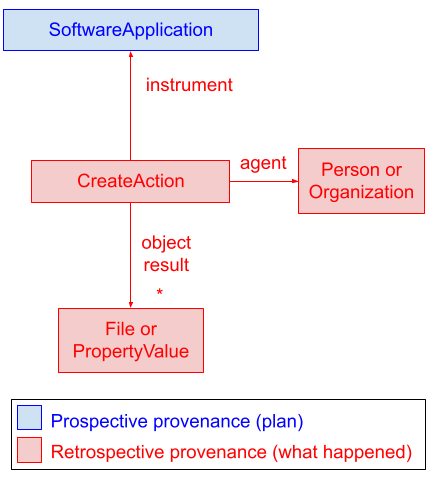
\includegraphics[width=21em]{image4.png}
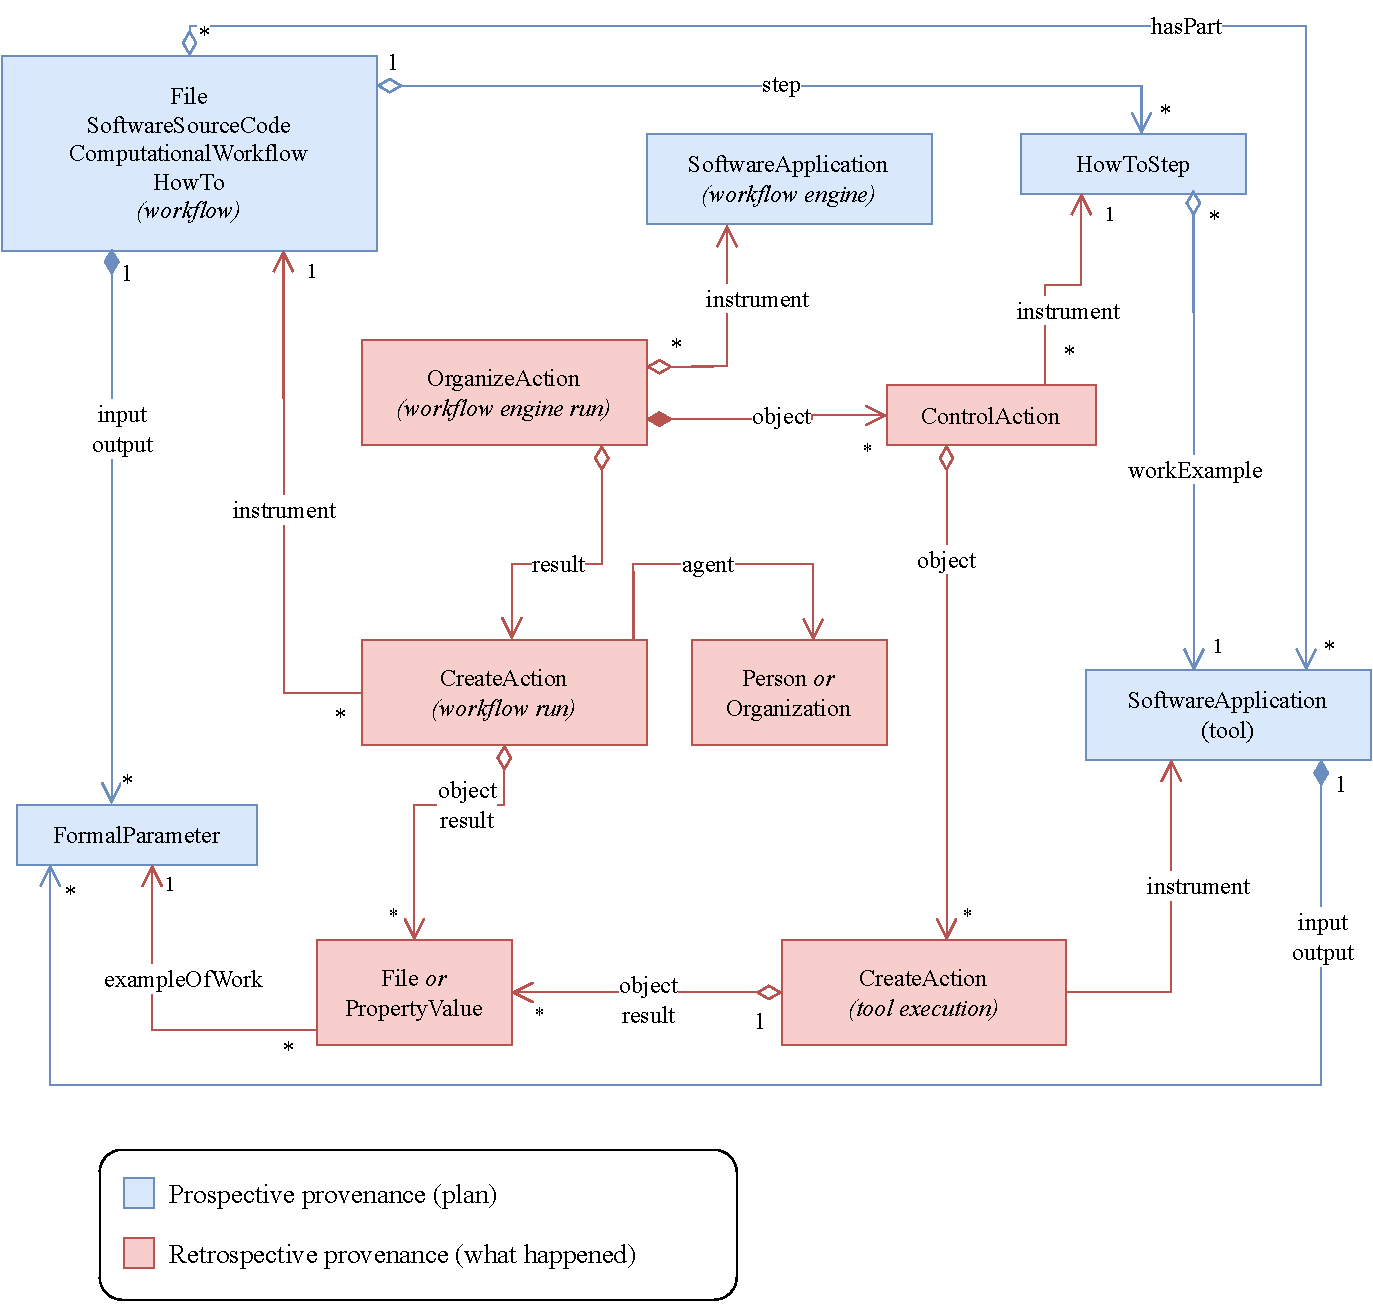
\includegraphics[width=\textwidth]{figures/ch54/wrroc-figure3.drawio.pdf}
%\includegraphics[width=\textwidth]{provenance_crate_er.eps}
\caption[UML class diagram for Provenance Run Crate]{{\bf UML class diagram for Provenance Run Crate.}
In addition to the workflow run, this profile represents the execution of individual steps and their related tools.}
\label{ch54:fig:provenance_crate_er}
\end{figure}

This profile also includes specifications on how to describe connections between parameters.
Parameter connections -- a fundamental feature of computational workflows -- describe (i) how tools take as input the intermediate outputs generated by other tools and (ii) how workflow-level parameters are mapped to tool-level parameters.
For instance, consider again the workflow depicted in Figure~\vref{ch54:fig:head_sort},
and suppose it is implemented in a workflow language such as CWL. The workflow-level input (a text file) is connected to the input of the “head” tool wrapper, and the output of the latter is connected to the input of the “sort” tool wrapper.


A representation of parameter connections is particularly useful for traceability, since it allows to document the inputs and tools on which workflow outputs depend.
Since the current RO-Crate context has no suitable terms for the description of such relationships, 
we added appropriate ones to the aforementioned  ``workflow-run'' context extension (the \url{https://w3id.org/ro/terms/workflow-run\#} namespace):
a \emph{ParameterConnection} type with
\emph{sourceParameter} and \emph{targetParameter} attributes that respectively map to the source and target formal parameters, and a
\emph{connection} property to link from the relevant step or workflow to the \emph{ParameterConnection} instances.

This profile is the most detailed of the three, and offers the highest level of granularity. Fig.~\vref{ch54:fig:profile_venn} shows the relationship between the specifications of the profiles as a Venn diagram.

\begin{figure}[htp]
%  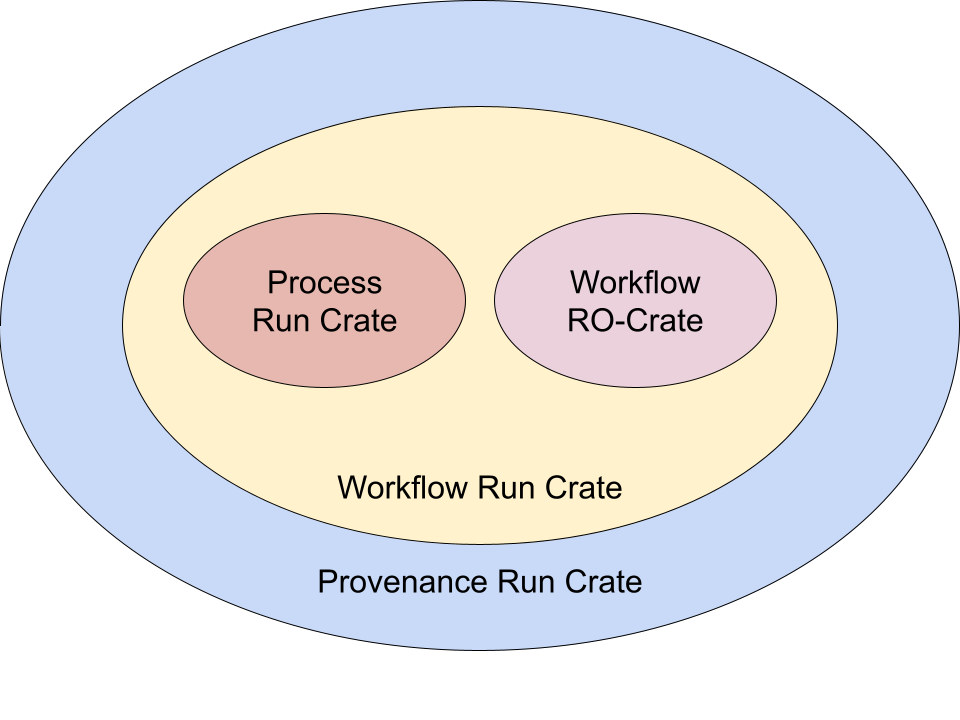
\includegraphics[width=21em]{venn.png}
  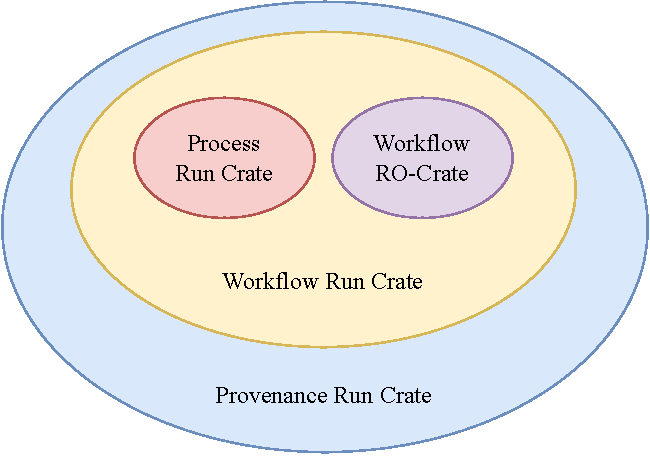
\includegraphics[width=26em]{figures/ch54/wrroc-venn.drawio.pdf}
  %\includegraphics[width=26em]{profile_venn.eps}
  \caption[Venn diagram of the specifications for the various RO-Crate profiles]{{\bf Venn diagram of the specifications for the various RO-Crate profiles.}
  Workflow Run Crate inherits the specifications of both Process Run Crate and Workflow RO-Crate. Provenance Run Crate, in turn, inherits the specifications of Workflow Run Crate.}
  \label{ch54:fig:profile_venn}
  \end{figure}


%%
\subsection{Implementations}\label{ch54:implementations}

Support for the Workflow Run RO-Crate profiles presented in this work has been implemented in a number of systems, showing support from the community and demonstrating their usability in practice.
We describe seven of these implementations (one in a conversion tool and six in WMS) in the following sections.
These tools have been developed in parallel by different teams, and independently from each other. 
RO-Crate has a strong ecosystem of tools \cite{Soiland-Reyes 2022} (section \vref{ch5:tooling}), and the WRROC implementations have either re-used these or added their own approach to the standards.


\subsubsection{Runcrate}\label{ch54:runcrate}

\footurl{https://github.com/ResearchObject/runcrate}{Runcrate} \cite{runcrate} is a Workflow Run RO-Crate toolkit which also serves as a reference implementation of the proposed profiles.
It consists of a Python package with a command line interface, providing a straightforward path to integration in Python software and other workflows.
The runcrate toolkit includes functionality to convert CWLProv ROs to RO-Crates conforming to the Provenance Run Crate profile (\emph{runcrate convert}), effectively providing an indirect implementation of the format for cwltool.
Indeed, the CWLProv model provided a basis for the Provenance Run Crate profile, and the implementation of a conversion tool in runcrate at times drove the improvement and extension of the profile as new requirements or gaps in the old designs emerged.
Runcrate converts both the retrospective provenance part of the CWLProv RO (the RDF graph of the workflow's execution) and the prospective provenance part (the CWL files, including the workflow itself).
Both parts are thus converted into a single, workflow language-agnostic metadata resource.

Another functionality offered by the runcrate package is \emph{runcrate report} which reports on the various executions described in an input RO-Crate, listing their starting and ending times, the values of the various parameters, etc. (example output in listing \vref{ch54:lst:ml_pipeline_streamflow_report}).
Runcrate report demonstrates how the provenance profiles presented in this work enable comparison of runs interoperably across different workflow languages or different implementations of the same language.
This functionality has also been used as a lightweight validator for the various implementations.

We also added a \emph{run} subcommand to re-execute the computation described by an input Workflow Run Crate or Provenance Run Crate where CWL was used as a workflow language.
It works by mapping the RO-Crate description of input parameters and their values (the workflow's
\emph{input} and the action's \emph{object}) to the format expected by CWL, which is then used to relaunch the workflow on the input data.
This functionality shows the machine-actionability of the profiles to support reproducibility, and was used to successfully re-execute the digital pathology annotation workflow described in section \vref{ch54:provenance-run-crate-for-digital-pathology}.

Of course, achieving a full re-execution in the general case may not always be possible: reproducibility is supported by the profiles, but also benefits from the characteristics of the workflow language (which should provide a clear formalism to map input items to their corresponding parameter slots) and from cooperation on the part of the workflow's author, who can help considerably by containerizing the environment required by each step and providing the relevant annotations (if allowed by the workflow language).


\subsubsection{Galaxy}\label{ch54:galaxy}

The Galaxy project~\cite{Galaxy 2022} provides a WMS with data management functionalities as a multi-user platform, aiming to make computational biology more accessible to research scientists that do not have computer programming or systems administration experience.
Galaxy's most prominent features include: a collection of 7500+ integrated \footurl{https://galaxyproject.org/toolshed/}{tools};
a web interface that allows the execution and definition of workflows using the integrated tools; a network of dedicated (public) Galaxy instances.

The export of workflow execution provenance data as Workflow Run Crates has been added in Galaxy's 23.0 release.
This feature provides a more interoperable alternative to the basic export of Galaxy workflow
\emph{invocations}: the workflow definition; a set of serialisations of the invocation-related metadata in Galaxy native, json-formatted files;
and the input and output data files.
This is achieved by extracting provenance from Galaxy entities related to the workflow run, along with associated metadata, converting them to RO-Crate metadata using the ro-crate-py library~\cite{ro-crate-py}; by describing all files contained in the basic invocation export within the RO-crate metadata;
and finally by making the Workflow Run Crate available for export to the user through Galaxy's web interface and API \cite{De Geest 2022}.

We extract the prospective provenance contained in Galaxy's YAML-based 
\footurl{https://galaxyproject.github.io/gxformat2/v19_09.html}{gxformat2} workflow definition, which includes details of the analysis pipeline such as the graph of tools that need to be executed, and metadata about the data types required.
The retrospective provenance -- i.e., the details of the executed workflow such as the inputs, outputs, parameter values used -- is extracted from Galaxy's data \footurl{https://docs.galaxyproject.org/en/master/lib/galaxy.model.html}{model}, which is not directly accessible to users in the context of a public Galaxy server.
All of this provenance information is then mapped to RO-Crate metadata, including some Galaxy-specific data entities such as dataset collections.
An exemplary exported Galaxy Workflow Run Crate is available on Zenodo~\cite{De Geest 2023b}.

In practice, a user would take the following steps to obtain a Workflow Run Crate from a Galaxy instance: 

\begin{enumerate}[(1)]
  \item Create or download a Galaxy workflow definition (e.g.: from WorkflowHub) and import it in a Galaxy instance, or create a workflow through the Galaxy GUI directly.
  \item Execute the workflow, providing the required inputs.
  \item After the workflow has run successfully, the corresponding RO-Crate will be available for export from the Workflow Invocations list.
\end{enumerate}


\subsubsection{COMPSs}\label{ch54:compss}

COMPSs~\cite{Lordan 2014} is a task-based programming model that allows users to transform a sequential application into a parallel one by simply annotating some of its methods, thus making it efficient to exploit the resources available (either distributed or in a cluster).
When a COMPSs application is executed, a corresponding workflow describing the application's tasks and their data dependencies is dynamically generated and used by the COMPSs runtime to orchestrate the execution of the application in the infrastructure.
As a WMS, COMPSs stands out for its many advanced features that enable applications to achieve fine-grained high efficiency in HPC systems, such as the ability to exploit underlying parallelisation frameworks (i.e.~MPI, OpenMP), compilers (e.g.~NUMBA), failure management, task grouping, and more.

Provenance recording for COMPSs workflows has been explored in previous work~\cite{Sirvent 2022}, where the Workflow RO-Crate profile was adopted in the implementation of a very lightweight approach to document provenance while avoiding the introduction of any significant run time performance overheads.
However, because of the dynamic nature of COMPSs workflows, the Workflow Run Crate profile is better suited to represent them, since workflows are created when the application is executed and, thus, a prior static workflow definition does not exist before that moment.
Due to this limitation, the workflow entity in the metadata file references the entry point application run by COMPSs, and formal parameters are not listed (note that listing them is not required by the profile) because inputs and outputs (both for each task and the whole workflow) are determined at runtime.
COMPSs is able to export provenance data with a post-processing operation that can be triggered at any moment after the application has finished.
The RO-Crate generation post-process uses information recorded by the runtime to detect and automatically add metadata of any input or output data assets used by the workflow.

Implementing Workflow Run Crate support in COMPSs required particular attention to the generation of a unique id for the \emph{CreateAction} representing the workflow run, combining hostname and queuing system job id for supercomputer executions (as extra information added), and just using generated UUIDs for distributed environments, to add as much information as available from the run while ensuring the id is unique.
In the \emph{CreateAction}, the \emph{description} term includes system information, as well as relevant environment variables that provide details on the execution environment (e.g., node list, CPUs per node).
Finally, the \emph{subjectOf} property of the \emph{CreateAction} references the system’s monitoring tool (when available),
where authorised users can see detailed profiling of the corresponding job execution, as provided by the MareNostrum IV \footurl{https://bsc.es/supportkc/docs/MareNostrum4/intro/}{supercomputer}.

To showcase the COMPSs adoption of the Workflow Run Crate profile, we provide as an example the execution of the BackTrackBB~\cite{Poiata 2016}
application in the MareNostrum IV supercomputer.
BackTrackBB targets the detection and location of seismic sources using the statistical coherence of the wave field recorded by seismic networks and antennas.
The resulting RO-Crate~\cite{Poiata 2023} complies with the Workflow Run Crate profile, and includes the application source files, a diagram of the workflow's graph, application profiling and input and output files.

The implementation of provenance recording following Workflow Run Crate has been fully integrated in the COMPSs runtime, and is available since \footurl{https://github.com/bsc-wdc/compss/tree/3.2}{release 3.2} \cite{Ejarque 2023}.


\subsubsection{StreamFlow}\label{ch54:streamflow}

The \footurl{https://github.com/alpha-unito/streamflow}{StreamFlow} framework~\cite{Colonnelli 2021} is a container-native WMS based on the CWL standard.
It has been designed around two primary principles: first, it allows the execution of tasks in multi-container environments, supporting the concurrent execution of communicating tasks in a multi-agent ecosystem; second, it relaxes the requirement of a single shared data space, allowing for hybrid workflow executions on top of multi-cloud, hybrid cloud/HPC, and federated infrastructures.
StreamFlow orchestrates hybrid workflows by combining a \emph{workflow description} (e.g., a CWL workflow description and a set of input values) with one or more \emph{deployment descriptions} -- i.e.
representations of the execution environments in terms of infrastructure-as-code (e.g., Docker Compose files \cite{Reis 2022}, HPC batch scripts, and Helm charts \cite{Zerouali 2023}).
A \texttt{streamflow.yml} file -- the entry point of each StreamFlow execution -- binds each workflow step with the set of most suitable execution environments.
At execution time, StreamFlow automatically takes care of all the secondary aspects, like scheduling, checkpointing, fault tolerance, and data movements.

StreamFlow stores prospective and retrospective provenance data in a proprietary format into a persistent pluggable database (using sqlite3 as the default choice).
After a CWL workflow execution completes, users can generate an RO-Crate through the \texttt{streamflow prov <workflow\_name>}
command, which extracts the provenance data stored in the database for one or more workflow executions and converts it to an RO-Crate archive that is fully compliant with the Provenance Run Crate Profile, including the details of each task run by the WMS.
Support for the format has been integrated into the main development branch and will be included in release 0.2.0 \cite{Colonnelli 2023b}.

From the StreamFlow point of view, the main limitation in the actual version of the Provenance Run Crate standard is the lack of support for distributed provenance, i.e., a standard way to describe the set of locations involved in a workflow execution and their topology. As a temporary solution,
the StreamFlow configuration and a description of the hybrid execution environment are preserved by directly including the \texttt{streamflow.yml} file into the generated archive.
However, this product-specific solution prevents a wider adoption from other WMS and forces agnostic frameworks (e.g., WorkflowHub) to provide ad-hoc plugins to interpret the StreamFlow format.
Since the support for hybrid and cross-facility workflows is gaining traction in the WMS ecosystem, we envision support for distributed provenance as a feature for future versions of Workflow Run RO-Crate.

\subsubsection{WfExS-backend}\label{ch54:wfexs}

\footurl{https://github.com/inab/WfExS-backend}{WfExS-backend} is a FAIR workflow execution orchestrator that aims to address some of the difficulties found in analysis reproducibility and analysis of sensitive data in a secure manner.
WfExS-backend requires that the software used by workflow steps is available in publicly available software containers for reproducibility.
Actual workflow execution is delegated to one of the supported workflow engines which matches with the workflow, right now either Nextflow or cwltool.
The orchestrator prepares and stages all the elements needed to run the workflow -- i.e. all the files of the workflow itself, the specific version of the workflow engine, the required software containers and the inputs.
All these elements are referred through resolvable identifiers, ideally public, permanent ones.
Due to this, the orchestrator can consume workflows which are originally available in different kinds of locations, like git repositories, Software Heritage, or even RO-Crates from WorkflowHub.

WfExS-backend development milestones aim to reach FAIR workflow execution through the generation and consumption of RO-Crates following the latest Workflow Run Crate profiles, which have proven to be a mechanism suitable to semantically describe digital objects in a way that simplifies embedding key details involved in analysis reproducibility and replicability.

The orchestrator records details relevant to the prospective provenance when a workflow is prepared for execution, such as the public URLs used to fetch input data and workflows, content digestion fingerprints (typically sha256 checksums) and metadata derived from workflow files, container images and input files.
Most of this metadata is represented in the generated RO-Crates. WfExS-backend has explicit commands to generate and publish both prospective and retrospective provenance RO-Crates based on a given existing staged execution scenario.
These RO-Crates can selectively include copies of used elements as payloads.
Workflows can be executed more than once in the same staged directory, with all the executions sharing the same inputs.
Thus, run details from all the executions are represented in the retrospective provenance RO-Crate. Support for Workflow Run RO-Crate is available since WfExS-backend version 0.10.1 \cite{Fernández 2023a}.
Future developments will also add support for embedding URLs of output results that have been deposited into a suitable repository (like Zenodo DOIs, for instance) as well as consuming previously produced RO-Crates.

An example of Workflow Run Crate generated by WfExS-backend from a Nextflow workflow run \cite{Bouyssié 2023} is available from Zenodo \cite{Fernández 2023b}.


\subsubsection{Sapporo}\label{ch54:sapporo}

Sapporo~\cite{Suetake 2022a} is an implementation of the Workflow Execution Service (WES) API \footurl{https://www.ga4gh.org/product/workflow-execution-service-wes/}{specification}.
WES is a standard proposed by the Global Alliance for Genomics and Health (GA4GH) for cloud-based data analysis platforms that receive requests to execute workflows.
Sapporo supports the execution of several workflow engines, including cwltool \cite{Amstutz 2023}, Toil \cite{Vivian 2017}, and StreamFlow \cite{Colonnelli 2021}.
Sapporo includes features specifically tailored to bioinformatics applications, including the calculation of feature statistics from specific types of outputs generated by workflow runs.
For example, the system calculates the mapping rate of DNA sequence alignments from BAM format files.
To describe the feature values, Sapporo uses the Workflow Run Crate profile extended with additional terms to represent these biological \footurl{https://github.com/ResearchObject/ro-terms/tree/master/sapporo}{features}.

Further, the Tonkaz companion command line software has integrated functionality to compare Run Crates generated by Sapporo to measure the reproducibility of the workflow outputs~\cite{Suetake 2023}.
Developers can use this unique feature to build a CI/CD platform for their workflows to ensure that changes to the product do not produce an unexpected result.
Workflow users can also use this feature to verify the results from the same workflow deployed in different environments.

While Sapporo supports Workflow Run Crate, since WES is a WMS wrapper, it does not parse the provided workflow definition files. 
Instead, it embeds the information in the files passed by the WES request to record the provenance of execution rather than using the actual workflow parameters meant for the wrapped WMS.
Therefore, the current implementation of Sapporo does not capture the connections between the inputs/outputs depicted in the workflow and the actual files used/generated during the run.
Thus, the profile generated by Sapporo has fields representing input and output files, but they are not linked to formal parameters.

Sapporo supports export to Workflow Run Crate since release 1.5.1 \cite{Suetake 2023b}. An example of RO-Crate generated by Sapporo is available on Zenodo \cite{Ohta 2023}.

\subsubsection{Autosubmit}\label{ch54:autosubmit}

Autosubmit~\cite{Manubens-Gil 2016} is an open source lightweight workflow manager and meta-scheduler created in 2011 for use in climate research to configure and run scientific experiments.
It supports scheduling jobs via SSH to Slurm~\cite{Yoo 2003}, PBS~\cite{Feng 2007} and other remote batch servers used in HPC.

The ``archive'' feature was added in \footurl{https://earth.bsc.es/gitlab/es/autosubmit/-/tags/v3.1.0}{Autosubmit 3.1.0}, released in 2015.
This feature archives the experiment directory and all its contents into a ZIP file, which can be used later to access the provenance data or to execute the Autosubmit experiment again.
Even though the data in the ZIP file includes prospective provenance and retrospective provenance, it contains no structure, and users have no way to tell which is which from just looking at the ZIP file and its contents.

Recent releases of Autosubmit 4 include an updated YAML configuration management system that allows users to combine multiple YAML files into a single unified configuration file.
While this gave users flexibility, it also increased the complexity to track the configuration changes and to relate these to the provenance data.
Another feature added in Autosubmit 4 is the option to use only the experiment manager features of Autosubmit, delegating the workflow execution to a different backend workflow engine, like ecFlow~\cite{Bahra 2011}, Cylc~\cite{Oliver 2019}, or a CWL runner.

In order to give users a more structured way to archive provenance, which includes the complete experiment configuration and the parameters used to generate the unified experiment configuration, and also to allow interoperability between workflow managers, the archive feature received a new flag in Autosubmit 4.0.100 \cite{Beltrán 2023} to generate Workflow Run RO-Crates.

The prospective provenance data is extracted from the Autosubmit experiment configuration.
This includes the multiple YAML files, and the unified YAML configuration, as well as the parameters used to preprocess each file -- preprocessing replaces placeholders in script templates with values from the experiment configuration.
The retrospective provenance data is included with the RO-Crate archive and includes logs and other traces produced by the experiment workflow.
Both prospective and retrospective provenance data are included in the final RO-Crate JSON-LD metadata file. Autosubmit uses the Workflow Run RO-Crate profile.

As one of the most recent implementations, much of the code added in Autosubmit 4 for RO-Crates was adapted from existing implementations like COMPSs and StreamFlow.
ro-crate-py~\cite{ro-crate-py} was used for the heavy lifting work of creating the RO-Crate archive in Python, and adding information for the JSON-LD metadata.

The main challenges for adopting RO-Crate in Autosubmit were incorporating Autosubmit's ``Project'' feature, and the lack of validation tools and of documentation and examples on how to use the standard with \emph{coarse-grained} workflow management systems (as described in~\cite{Goble 2020}) that do not track inputs and outputs, which is the case of Autosubmit -- as well as the Cylc and ecFlow workflow engines.

A Project in Autosubmit is an abstract concept that has a type and a location, and is used to separate experiment configuration and template scripts and other auxiliary files
The type can be Git, Subversion, or Local.
For each type the location represents the URL of a code repository, or a directory on a workstation or HPC file system used to copy the Project and its template scripts (written in Shell, R, or Python) and any other files (input data for a model, extra configuration files, binaries, etc.).
The workflows in Autosubmit have tasks with dependencies to other tasks, and each of these tasks execute one of these template scripts.
The RO-Crate file generated by Autosubmit includes only the project type and location, and not the complete Project.
Therefore, users have the provenance of the Project, but only those with the correct permissions can access its constituent resources (many applications run with Autosubmit can not be publicly shared without consent).

Validation tools for RO-Crate archives are still under development, and while there is a community-based review process to help and guide new implementations, a tool that others can use as code is written will contribute to a more agile development.

After working with the RO-Crate community on these issues, the Autosubmit team adopted a mixed approach where Autosubmit initialises the JSON-LD metadata from its configuration and local trace files, and the user is responsible for providing a partial JSON-LD metadata object in the Autosubmit YAML configuration.
A pull request was created to ro-crate-py to allow the RO-Crate JSON-LD metadata to be patched by these partial JSON-LD metadata objects.
This way, users are able to provide the missing information from the Autosubmit configuration model, like licence, authors, inputs, outputs, formal parameters, and more.
And by modifying ro-crate-py, future implementers of RO-Crate that have a similar workflow configuration as Autosubmit should be able to re-use it, while also using COMPSs, StreamFlow, Autosubmit, and other implementations as reference.

A workflow was created using an example Autosubmit Project~\cite{Kinoshita 2023} designed using UFZ's mHM (mesoscale Hydrological Model)
\cite{Samaniego 2010,Kumar 2013}. This workflow was used to validate the RO-Crate produced by Autosubmit.
This validation was performed by the Workflow Run RO-Crate community in a public GitHub \footurl{https://github.com/ResearchObject/workflow-run-crate/}{repository} and also using the aforementioned Runcrate.


\subsubsection{Summary of implementations}

Table \vref{ch54:implementation_summary_table} shows an overview of the different implementations presented in this section.


\begin{table}[htp]
%  \begin{adjustwidth}{-1.4cm}{0in} % Comment out/remove adjustwidth environment if table fits in text column.
  %\centering
  \begin{tabular}{l|l|l|l}
  \hline
  {\bf Impl.} & {\bf Profile} & {\bf Version URL/DOI} &
  {\bf Example}\\
  \hline
  runcrate & Provenance & \footnotesize \cite{runcrate}  & \footnotesize \cite{run-pathology} \\
  Galaxy & Workflow & \footnotesize \cite{Afgan 2023} & \footnotesize \cite{De Geest 2023b} \\
  COMPSs & Workflow & \footnotesize \cite{Ejarque 2023} & \footnotesize \cite{Poiata 2023} \\
  Streamflow & Provenance & \footnotesize \cite{Colonnelli 2023b} & \footnotesize \cite{Colonnelli 2023} \\
  WfExS & Workflow & \footnotesize \cite{Fernández 2023a} & \footnotesize \cite{Fernández 2023b} \\
  Sapporo & Workflow & \footnotesize \cite{Suetake 2023b} & \footnotesize \cite{Ohta 2023} \\
  Autosubmit & Workflow & \footnotesize \cite{Beltrán 2023} & \footnotesize \cite{Kinoshita 2023} \\
  \end{tabular}
  %\begin{flushleft} 
    
\caption[Workflow Run Crate implementations]{{\bf Workflow Run Crate implementations}. Summary of each WRROC implementation, together with the profiles it implements, the latest software citation and an example crate of its application. Runcrate is a toolkit that converts CWLProv ROs to Provenance Run Crates, while the others are WMS.}
  %\end{flushleft}
  \label{ch54:implementation_summary_table}
 % \end{adjustwidth}
\end{table}
  


%% 
\subsection{Exemplary Use Cases}\label{ch54:exemplary-use-cases}

We illustrate Workflow Run RO-Crate on two exemplary use cases, which are similar in terms of application domain -- machine learning-aided tumour detection in human prostate images -- but quite different in the way computations are executed and provenance is represented: in the first, the analysis is conducted by means of a CWL workflow and the outcome is represented with Provenance Run Crate; in the second, a combination of Process Run Crate and CPM RO-Crate is used to represent a sequence of computations linked to their corresponding CPM provenance information.


\subsubsection{Provenance Run Crate for Digital Pathology}\label{ch54:provenance-run-crate-for-digital-pathology}

We present a use case that demonstrates the effectiveness of our most detailed profile Provenance Run Crate at recording provenance data in the context of digital pathology.
More specifically, we demonstrate the generation of RO-Crates to save provenance data associated with the computational annotation of magnified prostate tissue areas and cancer subregions using deep learning models~\cite{Del Rio 2022}.
The image annotation process is implemented in a CWL workflow consisting of three steps, each executing inference on an image using a deep learning model: inference of a low-resolution tissue mask to select areas for further processing;
high-resolution tissue inference on areas identified in the previous step to refine borders; high-resolution cancer identification on areas identified in the first step.
The two tissue inference steps run the same tool, but set different values for the parameter that controls the magnification level.
The workflow is integrated in the 
\footurl{https://github.com/crs4/DigitalPathologyPlatform}{CRS4 Digital Pathology Platform}, a web-based platform to support clinical studies involving the examination and/or the annotation of digital pathology images.

To assess the interoperability of WRROC, we recorded the provenance of the same exemplary workflow in two different execution platforms.
In the first case, the workflow was executed with the StreamFlow WMS, for which the Provenance Run Crate implementation is discussed in Section \vref{ch54:streamflow}.
In the second case, we executed the CWL workflow with cwltool and converted the resulting CWLProv RO to a Provenance Run Crate with the runcrate tool (Section \vref{ch54:runcrate}).

The RO-Crates obtained in the two cases~\cite{Colonnelli 2023, run-pathology}
are very similar to each other, differing only in a few details: for instance,~\cite{Colonnelli 2023} includes the StreamFlow configuration file and has separate files for the workflow and the two tools, while
\cite{run-pathology} has the workflow and the tools stored in a single file (CWL's ``packed'' format).
Apart from these minor differences, the description of the computation is essentially the same.

Four actions are represented: the workflow itself, the two executions of the tissue extraction tool and the execution of the tumour classification tool.
Each action is linked to the corresponding workflow or tool via the
\emph{instrument} property, and reports its starting and ending time. For each action, input and output slots are referenced by the workflow, while the corresponding values are referenced by the action itself.
The data entities and \emph{PropertyValue} instances corresponding to the input and output values link to the corresponding parameter slots via the \emph{exampleOfWork} property, providing information on the values taken by the parameters.

Listing~\vref{ch54:lst:ml_pipeline_streamflow_report} shows the output of the
\texttt{runcrate report} command for the StreamFlow RO-Crate. 
For each action (workflow or tool run), the tool reports the associated instrument (workflow or tool), the starting and ending time and the list of inputs and outputs, with arrows pointing from the formal parameter to the corresponding actual value taken during the execution of the action.

\begin{listing}
%\begin{adjustwidth}{-0.5cm}{0in}
  \caption[runcrate report command line output]{\texttt{runcrate report} command line output. This informal listing of relevant RO-Crate entities describe each step execution. Note that inputs and outputs are of different types (not shown), e.g. \texttt{tissue\_low>0.9} is a string parameter, \texttt{6b15de…} is a filename, and \texttt{\#af0253…} is a collection.}
  \label{ch54:lst:ml_pipeline_streamflow_report}
\begin{footnotesize}
\begin{verbatim}
action: #30a65cba-1b75-47dc-ad47-1d33819cf156
  instrument: predictions.cwl (['SoftwareSourceCode', 
         'ComputationalWorkflow', 'HowTo', 'File'])
  started: 2023-05-09T05:10:53.937305+00:00
  ended: 2023-05-09T05:11:07.521396+00:00
  inputs:
    #af0253d688f3409a2c6d24bf6b35df7c4e271292 <- predictions.cwl#slide
    tissue_low <- predictions.cwl#tissue-low-label
    9 <- predictions.cwl#tissue-low-level
    tissue_low>0.9 <- predictions.cwl#tissue-high-filter
    tissue_high <- predictions.cwl#tissue-high-label
    4 <- predictions.cwl#tissue-high-level
    tissue_low>0.99 <- predictions.cwl#tumor-filter
    tumor <- predictions.cwl#tumor-label
    1 <- predictions.cwl#tumor-level
  outputs:
    06133ec5f8973ec3cc5281e5df56421c3228c221 <- predictions.cwl#tissue
    4fd6110ee3c544182027f82ffe84b5ae7db5fb81 <- predictions.cwl#tumor
action: #457c80d0-75e8-46d6-bada-b3fe82ea0ef1
  step: predictions.cwl#extract-tissue-low
  instrument: extract_tissue.cwl (['SoftwareApplication', 'File'])
  started: 2023-05-09T05:10:55.236742+00:00
  ended: 2023-05-09T05:10:55.910025+00:00
  inputs:
    tissue_low <- extract_tissue.cwl#label
    9 <- extract_tissue.cwl#level
    #af0253d688f3409a2c6d24bf6b35df7c4e271292 <- extract_tissue.cwl#src
  outputs:
    6b15de40dd0ee3234062d0f261c77575a60de0f2 <- extract_tissue.cwl#tissue
action: #d09a8355-1a14-4ea4-b00b-122e010e5cc9
  step: predictions.cwl#extract-tissue-high
  instrument: extract_tissue.cwl (['SoftwareApplication', 'File'])
  started: 2023-05-09T05:10:58.417760+00:00
  ended: 2023-05-09T05:11:03.153912+00:00
  inputs:
    tissue_low>0.9 <- extract_tissue.cwl#filter
    6b15de40dd0ee3234062d0f261c77575a60de0f2 <- extract_tissue.cwl#filter_slide
    tissue_high <- extract_tissue.cwl#label
    4 <- extract_tissue.cwl#level
    #af0253d688f3409a2c6d24bf6b35df7c4e271292 <- extract_tissue.cwl#src
  outputs:
    06133ec5f8973ec3cc5281e5df56421c3228c221 <- extract_tissue.cwl#tissue
action: #ae2163a8-1a2a-4d78-9c81-caad76a72e47
  step: predictions.cwl#classify-tumor
  instrument: classify_tumor.cwl (['SoftwareApplication', 'File'])
  started: 2023-05-09T05:10:58.420654+00:00
  ended: 2023-05-09T05:11:06.708344+00:00
  inputs:
    tissue_low>0.99 <- classify_tumor.cwl#filter
    6b15de40dd0ee3234062d0f261c77575a60de0f2 <- classify_tumor.cwl#filter_slide
    tumor <- classify_tumor.cwl#label
    1 <- classify_tumor.cwl#level
    #af0253d688f3409a2c6d24bf6b35df7c4e271292 <- classify_tumor.cwl#src
  outputs:
    4fd6110ee3c544182027f82ffe84b5ae7db5fb81 <- classify_tumor.cwl#tumor
\end{verbatim}
\end{footnotesize}
%\end{adjustwidth}
\end{listing}


The \emph{exampleOfWork} link between input / output values and parameter slots is used by \texttt{runcrate run} to reconstruct the CWL input parameters document needed to rerun the computation.
The
\emph{alternateName} property (a Schema.org property applicable to all entities), which records the original name of data entities (at the time the computation was run), is also crucial for reproducibility in this case: both StreamFlow and CWLProv, to avoid clashes, record input and output files and directories using their SHA1
checksum as their names. 
However, this particular workflow expects the input dataset to be in the \footurl{https://openslide.org/formats/mirax/}{MIRAX} format, where the ``main'' file taken as an input parameter by the processing application must be accompanied by a directory in the same location with the same name apart from the extension.
The runcrate tool uses the \emph{alternateName} to rename the input dataset as required, so that the expected pattern can be picked up by the workflow during the re-execution.
This use case was the main motivation to include a recommendation to use \emph{alternateName} with the above semantics in Process Run Crate.

Thanks to the fact that both RO-Crates were generated following the best practices to support reproducibility mentioned in the profiles, we were able to re-execute both computations with the runcrate tool.
This was also made possible by the fact that the CWL workflow included information on which container images to use for each tool.
Overall, this shows how reproducibility is a hard-to-achieve goal that can only be supported, but not ensured, by the profiles, since it also depends on factors like the characteristics of the computation, the choice of workflow language and whether best practices such as containerisation are followed.

This use case highlighted the need to add specifications on how to represent multi-file datasets \cite[section Representing multi-file objects]{WRROC 2023a}. In the MIRAX format, in fact, the ``main'' file must be accompanied by a directory in the same location containing additional files with a specific structure.
To represent this, we added specifications to the Process Run Crate profile on \footurl{https://w3id.org/ro/wfrun/process/0.4\#representing-multi-file-objects}{describing “composite” datasets} consisting of multiple files and directories to be treated as a single unit -- as opposed to more conventional input or output parameters consisting of a single file. The profile specifies that such datasets should be represented by a \emph{Collection} entity linking to individual files and directories via the \emph{hasPart} property, and referencing the main part (if any) via the \emph{mainEntity} property. Note that, by adding this specification to Process Run Crate, we also made it available to Workflow Run Crate and Provenance Run Crate. In the output of the runcrate report tool the additional files are not shown, since the formal parameter points to the \emph{Collection} entity that describes the whole dataset.

\subsubsection{Process Run Crate and CPM RO-Crate for cancer detection}\label{ch54:process-run-crate-and-cpm-ro-crate-for-cancer-detection}

This section presents an RO-Crate created to describe an execution of a computational pipeline that trains AI models to detect the presence of carcinoma cells in high-resolution digital images of magnified human prostate tissue.
The RO-Crate makes use of Process Run Crate and CPM RO-\footurl{https://w3id.org/cpm/ro-crate}{Crate}, an RO-Crate profile that supports the representation of entities described according to the Common Provenance Model (CPM) \cite{Wittner 2022,Wittner 2023b}. 

The CPM, an extension of the W3C PROV model \cite{Moreau 2013} is a recently developed provenance model that enables the representation of distributed provenance. 
Distributed provenance is created when an object involved in the research process, either digital or physical (e.g., biological material), is exchanged between organisations, so that each organisation can document only a portion of the object’s life cycle. 
Individual provenance components are generated, stored, and managed individually by each organisation, and are linked together in a chain. 
The CPM prescribes how to represent such provenance, and how to enable its traversal and processing using a common algorithm, independently from the type of object being described. 
In addition, the CPM defines a notion of meta-provenance, which contains metadata about the history of individual provenance components. 

CPM RO-Crate supports the identification of CPM-based provenance and meta-provenance files within an RO-Crate, allowing to pack data, metadata, and CPM-based provenance information together. 
An RO-Crate generated according to the CPM-RO-Crate profile embeds parts of the distributed provenance, which may be linked to the provenance of precursors and successors of the packed data. 

The CPM-RO-Crate profile synergises well with Process Run Crate, since the former can add references to CPM-based provenance descriptions of computational executions described with the latter, integrating them in the distributed provenance. Since CPM-based provenance and meta-provenance files are typically themselves produced by computations, Process Run Crate allows to represent these along with the main computations that produce the datasets being exchanged, providing the full picture in a cohesive ensemble.


The pipeline consists of three main computational steps: a preprocessing step that splits input images into small patches and divides them into a training and a testing set; a training step that trains the model to recognise the presence of carcinoma cells in the images; an evaluation step that measures the accuracy of the trained model on the testing set.
In addition to the pipeline steps, the RO-Crate describes additional computations related to the generation of the CPM provenance and meta-provenance files.
All computations are described according to the Process Run Crate profile, while the CPM files are referenced according to the CPM RO-Crate profile. 

Also represented via Process Run Crate are: the input dataset; the results of the pipeline execution; the scripts that implement the pipeline; the log files generated by the scripts; a script that converts the logs into the CPM files.
This allowed us to describe all involved elements as a single aggregate, with entities and their relationships represented according to the RO-Crate model.
The RO-Crate discussed here is available from Zenodo~\cite{Wittner 2023c}.

The CPM files complement the RO-Crate with internal details about the pipeline execution, such as how the input dataset was split into training and testing sets, or detailed information about each training iteration of the AI model.
For instance, it contains a representation of a checkpoint of the AI model after the second training iteration.
The corresponding entity's attributes contain paths to the respective model stored as a file.
The entity is related to the respective training iteration activity, which contains the iteration parameters represented as an attribute list.

In addition, the CPM generally provides means to link the input dataset provenance to the provenance of its precursors -- human prostate tissues and biological samples the tissues were derived from; this is not included in the example because we used a publicly available input database for which provenance of the precursors was not available.
However, the linking mechanism for provenance precursors is exactly the same as between the bundles for the AI pipeline parts.

While the RO-Crate is focused on the execution of the pipeline, the provenance included in the CPM files intends to be interlinked with provenance of the precursors or successors, providing means to traverse the whole provenance chain.
For the described digital pathology pipeline, the precursors would be: 

\begin{enumerate}[(1)]
  \item A biological sample acquired from a patient.
  \item Slices of the sample processed and put on glass slides.
  \item The images created as a result of scanning the slides using a microscope.
\end{enumerate}

As a result, combining the CPM and RO-Crate enables the lookup of research artefacts related to the computation across heterogeneous organisations using the underlying provenance chain.


%
\subsection{Discussion}\label{ch54:discussion}


The RO-Crate profiles presented here provide a unified data model to describe the prospective and retrospective provenance of the execution of a computational workflow, together with contextual metadata about the workflow itself and its associated entities (inputs, outputs, code, etc.). 
The profiles are flexible, allowing to tailor the description to a broad variety of use cases, agnostic with respect to the WMS used and allow describing provenance traces at different levels of granularity. 
This facilitates developing implementations by multiple workflow systems (often with heterogeneous assumptions and requirements) -- six of which have already been developed and are described in Section \vref{ch54:implementations} -- allowing to perform comparisons between runs across heterogeneous systems.
For instance, the \footurl{https://www.w3.org/TR/sparql11-overview/}{SPARQL} query in listing \vref{ch54:sparql} returns all actions in a Workflow Run RO-Crate, together with their instruments and their starting and ending times:

\begin{listing}
\begin{verbatim}
PREFIX schema: <http://schema.org/>
SELECT ?action ?instrument ?start ?end
WHERE {
  ?action a schema:CreateAction .
  ?action schema:instrument ?instrument .
  OPTIONAL { ?action schema:startTime ?start } .
  OPTIONAL { ?action schema:endTime ?end }
}
\end{verbatim}
\caption{SPARQL query to find actions in a Workflow Run RO-Crate}
\label{ch54:sparql}
\end{listing}

Additionally, having workflow runs and plans described according to the RO-Crate model allows capturing the context of the workflow itself (e.g.~authors, related publications, other workflows, etc.) rather than the trace alone. 
Being based on RO-Crate, the profiles and their implementations are part of a growing \footurl{https://www.researchobject.org/ro-crate/in-use/}{ecosystem} of tools and services maintained by the RO-Crate community. 

Another advantage of RO-Crate is that the files corresponding to the data entities (inputs, outputs, code, etc.) do not necessarily have to be stored together with the metadata file: for instance, they can be remote and referred to via an http(s) URI. This is mostly relevant in situations where the file is very large or cannot be shared publicly: the data entity's identifier can be a URI that is accessible only through authentication, or resolvable only within the boundaries of the generating organisation.

The derivation of Workflow Run Crate from Workflow RO-Crate and, in turn, of Provenance Run Crate from Workflow Run Crate makes RO-Crates that conform to these profiles compatible with the WorkflowHub workflow registry, allowing workflow runs to be registered and easily found and shared with other researchers. Additionally, the inheritance mechanism allows reusing the specifications already developed for Workflow RO-Crate, which form part of the guidelines on representing the prospective provenance

The Workflows Community Summit \cite{Ferreira 2022} identified as one of the current open challenges in the Scientific Workflows domain the ability to build FAIR into Workflow Management Systems, with the objective of achieving FAIR Computational Workflows. The profiles introduced in this article are able to help tackle this by introducing interoperable metadata among WMSs that captures the provenance of their corresponding workflow executions.

The Workflow Run RO-Crate profiles, the associated tooling, the implementations and the examples are developed by a community that runs regular virtual meetings (every two weeks at the time of writing) and coordinates on Slack and the RO-Crate mailing list.
The WRROC community brings together members of the RO-Crate community~\cite{Soiland-Reyes 2022}, WMS users and developers, Workflow users and developers, GA4GH~\cite{Rehm 2021} Cloud developers and provenance model authors, and is open to anyone who is interested in the representation of workflow provenance.
The inclusion of WMS developers and workflow users was key to keeping the specifications flexible, easy to implement and grounded on real use cases, while the diversity of the stakeholders allowed to keep a plurality of viewpoints while driving the model's development forward.

One of the main benefits of this development process is that the profiles are already in use, with seven implementations (six WMS and one conversion tool) already available as described in section \vref{ch54:implementations}.

In the following subsections, we provide an evaluation of the metadata coverage of runcrate and we discuss WRROC relates to standards such as W3C PROV and to other community projects.


\subsubsection{Evaluation of metadata coverage using runcrate convert}

In order to assess the metadata coverage of \emph{runcrate} (section \vref{ch54:runcrate}), we performed a qualitative analysis of the tool's \emph{convert} mode, in which we evaluated how the generated RO-Crates preserve the metadata contained in the CWLProv ROs from which they are derived.
For this analysis, we followed the same approach as for an earlier evaluation of CWLProv~\cite{de Wit 2022}.
In that work, we identified and analysed three levels of representation:
firstly, in RDF; secondly, in a structured, but CWL-specific document;
and finally, in an unstructured, human readable format.
From this earlier analysis, we concluded that the CWLProv RDF representation of the workflow runs lacked many provenance metadata that was included in CWL-specific documents, such as the packed workflow and input parameter file.
For example, the CWLProv RDF only contained the name of each workflow step, without including the link to the underlying CommandLineTool or nested Workflow that was executed; information that could be extracted from the packed workflow.

In our analysis of runcrate, we compared the CWLProv RDF provenance graph with the RO-Crate metadata file. The results of the analysis are summarised in Table
\vref{ch54:analysis_table} \footnote{
  The three dots (…) in the WRROC column indicate that  the concept is supported in an RO-Crate using existing schema.org vocabulary (e.g. \url{https://schema.org/softwareHelp}) but is not required or recommended by the WRROC profiles.
}.
Overall, most of the information contained in CWLProv RDF is transferred to the RO-Crate metadata.
In addition, the representation of some categories of metadata has improved, notably Workflow parameters (WF2), which were insufficiently described in CWLProv RDF but defined with type and format in RO-Crate.
Moreover, the format of input files (D2), which was partially represented in CWLProv RDF, is fully represented in RO-Crate.

% Place tables after the first paragraph in which they are cited.
\begin{table}[tp]
%\begin{adjustwidth}{-1.4cm}{0in} % Comment out/remove adjustwidth environment if table fits in text column.
\centering
\caption{Summarised results of our qualitative analysis of runcrate}
\begin{tabular}{r|l|l|c|c|c|c}
\hline
%% TODO: Check ticks are in right places
{\bf Type} & {\bf Subtype}      & {\bf Name} & {\bf CWL} & {\bf CWLProv} & {\bf RO-Crate} & {\bf WRROC}  \\ \hline
T1 & SC1 & Workflow design      & $\bullet$ &  $\cdot$ & $\circ$ & $\dots$ \\ 
& SC2 & Entity annotations      & $\cdot$ &  $\cdot$ &  $\cdot$  & $\dots$ \\ 
& SC3 & Workflow execution ann. &  $\cdot$  & $\cdot$ &  $\cdot$ & $\dots$ \\ \hline
T2 & D1 & Data identification   & $\circ$ & $\cdot$ &  $\cdot$ & $\dots$ \\
& D2 & File characteristics     & $\circ$ & $\circ$ & $\bullet$ & $\circ$ \\
& D3 & Data access              & $\circ$ &  $\cdot$ &  $\cdot$  & $\dots$ \\ 
& D4 & Parameter mapping        & $\bullet$ & $\bullet$ & $\bullet$ & $\bullet$ \\ \hline 
T3 & SW1 & Software identification & $\circ$ &  $\cdot$ & $\circ$ & $\dots$ \\ 
& SW2 & Software documentation  & $\cdot$ &  $\cdot$ & $\cdot$ & $\dots$ \\  
& SW3 & Software access         & $\cdot$ &  $\cdot$ & $\cdot$ & $\dots$ \\ \hline 
T4 & WF1 & Workflow software    & $\bullet$ & $\circ$ & $\circ$ & $\dots$ \\ 
& WF2 & Workflow parameters     & $\bullet$ & $\circ$ & $\bullet$ & $\bullet$ \\ 
& WF3 & Workflow requirements   & $\bullet$ &  $\cdot$  &  $\circ$  & $\circ$ \\ \hline 
T5 & ENV1 & Software environment & $\cdot$ & $\cdot$ &  $\cdot$ & $\cdot$ \\ 
& ENV2 & Hardware environment   & $\cdot$ & $\cdot$ &  $\cdot$  & $\cdot$\\ 
& ENV3 & Container image        & $\circ$ & $\circ$ &  $\circ$ & $\bullet$ \\ \hline 
T6 & EX1 & Execution timestamps & $\cdot$ & $\bullet$ & $\bullet$ & $\bullet$ \\ 
& EX2 & Consumed resources      & $\cdot$ & $\cdot$ & $\cdot$ & $\cdot$  \\ 
& EX3 & Workflow engine         & $\cdot$ & $\circ$ & $\circ$ & $\circ$  \\  
& EX4 & Human agent             & $\cdot$ & $\bullet$ & $\bullet$ & $\bullet$ \\ \hline
\end{tabular}
\begin{flushleft}
  \small We compared RO-Crates with the CWLProv ROs from which they were generated.
The analysis was based on a provenance taxonomy reflecting relevant provenance metadata based on realistic use cases for ROs associated with a real-life bioinformatics workflow \cite{de Wit 2022}.
CWL-specific documents are: \texttt{packed.cwl} (the workflow), \texttt{primary-job.json} (the inputs file), and \texttt{primary-output.json} (the outputs file).
Since \texttt{packed.cwl} is also included in RO-Crate, we only considered how the metadata was represented in \texttt{ro-crate-metadata.json}.\\
For completeness we also show the theoretical capability of the Provenance Run Crate profile (WRROC column) assuming all its MUST/SHOULD requirements are complete.
The categories in the first three columns are explained in \cite{de Wit 2022}.
\\
\textbf{Legend:} $\bullet$ fully represented  $\;\;\circ$ partially represented   $\;\;\cdot$ missing or unstructured representation $\;\;\dots$ optional (e.g. schema.org attribute)
\end{flushleft}
\label{ch54:analysis_table}
%\end{adjustwidth}
\end{table}

In conclusion, our analysis shows that runcrate preserves most provenance metadata previously shown to be relevant in realistic RO use case scenarios.
The full results of the analysis can be found in \cite{de Wit 2023}.

From this analysis it is worth highlighting the gaps and potential for Workflow Run RO-Crates. Several areas have been flagged by this study as important aspects of workflow metadata, such as Data Access (D3), Software Documentation (SW2) and Workflow Requirements (WF3). Many such aspects require human annotation and cannot be provided by workflow engines alone, although they may be propagated from workflow and tool definitions. Some areas like Consumed Resources (EX2) require additional terms to be defined, and are part of future work.


\subsubsection{Workflow Run RO-Crate and the W3C PROV standard}
\label{ch54:prov}

Our aim is to be compatible with both Schema.org and W3C PROV. Provenance Run Crate is the profile that most closely matches the level of detail provided by CWLProv, which extends W3C PROV. Table \vref{ch54:rocrate_prov_mapping} shows how the main entities and relationships represented by Provenance Run Crate map to PROV constructs, using the SKOS vocabulary to indicate the type of relationship between each pair of terms. A machine-readable version of the mapping can be found in the \footurl{https://w3id.org/ro/doi/10.5281/zenodo.10368989}{accompanying RO-Crate} of this article \cite{wrroc-crate}.

\begin{table}[p]
  %\begin{adjustwidth}{-2.25in}{0in} % Comment out/remove adjustwidth environment if 
  %\begin{adjustwidth}{-1.5cm}{0in}
  \centering
  \caption[Mapping from Workflow Run RO-Crate to equivalent W3C PROV concepts]{
  {\bf Mapping from Workflow Run RO-Crate to equivalent W3C PROV concepts} using SKOS \cite{w3-skos-primer}. For instance, \emph{CreateAction} has \textbf{broader} match PROV's \emph{Activity}, meaning that \emph{Activity} is more general.}
  \begin{tabular}{p{40mm}|p{50mm}|p{40mm}}
  \hline
%  {\bf W3C PROV} & {\bf RO-Crate} & \textbf{Relationship} \\
  {\bf RO-Crate} & \textbf{Relationship} & {\bf W3C PROV-O} \\
  \hline

  \emph{Action} (superclass of \emph{CreateAction}, \emph{OrganizeAction}) & 
    Has close match 
    \begin{small}
      (schema.org Actions may also be potential actions in the future)
    \end{small}
    & 
    \emph{Activity}
    \\ \hline
  \emph{CreateAction}, \emph{OrganizeAction} & 
    Has broader match & 
    \emph{Activity}
    \\ \hline
  \emph{Person} & 
    Has exact match & 
    \emph{Person}
    \\ \hline
  \emph{Organization} & 
    Has exact match & 
    \emph{OrganizeAction} 
    \\ \hline
  \emph{SoftwareApplication} & 
    Has related match & 
    \emph{SoftwareAgent}
    \\ \hline
  \emph{ComputationalWorkflow}, \emph{SoftwareApplication}, \emph{HowTo} & 
    Has broader match & 
    \emph{Plan},
    \emph{Entity}
    \\ \hline
  \emph{File}, \emph{Dataset}, \emph{PropertyValue} & 
    Has broader match & 
    \emph{Entity}
    \\ \hline
  \emph{startTime} on \emph{CreateAction} & 
    Has close match & 
    \emph{startedAtTime}
    \\ \hline
  \emph{endTime} on \emph{CreateAction} & 
    Has close match & 
    \emph{endedAtTime}
    \\ \hline
  \emph{agent} on \emph{CreateAction} & 
    Has related match & 
    \emph{wasStartedBy}, \emph{wasEndedBy}
    \\ \hline
  \emph{agent} and \emph{instrument} on \emph{CreateAction} & 
    Has broader match & 
    \emph{wasAssociatedWith}
    \\ \hline
  \emph{instrument} on \emph{CreateAction} & 
    Has related match 
    \begin{small}
      (Complex mapping: an instrument implies a qualified association with the agent, linked to a plan)
    \end{small}
    & 
    \emph{hadPlan} on \emph{Association}
    \\ \hline

  \emph{object} on \emph{CreateAction} &
    Has exact match & 
    \emph{used} 
    \\ \hline
  \emph{result} on CreateAction & 
    Has close match & 
    inverse \emph{wasGeneratedBy} 
  
  \end{tabular}
  %\begin{flushleft} Table notes \end{flushleft}
  \label{ch54:rocrate_prov_mapping}
 % \end{adjustwidth}
\end{table}
  

\subsubsection{Five Safes Workflow Run Crate}\label{ch54:trusted-workflow-run-crate}

The \emph{Five Safes RO-Crate} \cite{5s-crate} profile has been developed to extend the Workflow Run RO- Crate profile for use in Trusted Research Environments (TRE) in order to handle sensitive health data in federated workflow execution across TREs in the UK \cite{trefx} and following the Five Safes Framework \cite{Desai 2016}.
A crate with a workflow run request references a pre-approved workflow and project details for manual and automated assessment according to the TRE's agreement policy for the sensitive dataset. 

The crate then goes through multiple phases internal to the TRE, including validation, sign-off, workflow execution and disclosure control \cite{Soiland-Reyes 2023f}.
At this stage the crate is also conforming to the Workflow Run Crate profile.
The final crate is then safe to be made public.
This extension of Workflow Run Crate documents and supports the \emph{human review process} -- important for transparency on TRE data usage. 
The initial implementation of this profile used WfExS as the workflow execution backend, and this approach will form the basis for further work on implementing federated workflow execution in the British initiatives DARE UK and \footurl{https://esciencelab.org.uk/projects/federated-analytics/}{HDR UK} \cite{Snowley 2023} and in the European \footurl{https://esciencelab.org.uk/projects/eosc-entrust/}{EOSC-ENTRUST} project for Trusted Research Environment.


\subsubsection{Biocompute Object RO-Crate}\label{ch54:bco-crate}
\cite{ieee2791}, colloquially \emph{Biocompute Objects} (BCO), is a standard for representing provenance of a genomic sequencing pipeline, intended for submission of the workflow to regulatory bodies, e.g. as part of a personalised medical treatment method \cite{Alterovitz 2018}. 
The BCO is represented as a single JSON file which includes description of the workflow and its steps and intended purpose, as well as references for tools used and data sources accessed. 
There is overlap in the goals of BCO and Workflow Run Crate profiles; however, their intentions and focus are different. 
BCO is primarily conveying a computational method for the purpose of manual regulatory review and further reuse, with any values provided as an exemplar run.  
A Workflow Run Crate, however, is primarily documenting a particular workflow execution, and the workflow is associated to facilitate rerun rather than reuse. 

Previously, a \footurl{https://biocompute-objects.github.io/bco-ro-crate/}{guide} to packaging BioCompute Objects using RO-Crate was developed as a profile to combine both standards \cite{Soiland-Reyes 2021}.
In this early approach, RO-Crate was primarily a vessel to transport the BCO along with its constituent resources, including the workflow and data files, as well as provide these resources with additional typing and licence metadata that is not captured by the BCO JSON. 
Further work is being planned with the BCO community to update the BCO-RO profile to align with the newer Workflow Run Crate profiles. 

\subsection{Conclusion and Future Work}\label{ch54:conclusion}

In this work we presented Workflow Run RO-Crate, a collection of RO-Crate profiles to represent the provenance of the execution of computational workflows at different levels of granularity.
We described each profile and their corresponding implementations, shown how they apply to real use cases and described the community behind their development process.
Workflow Run RO-Crate has already been adopted by six WMS, including Galaxy, StreamFlow and COMPSs. The flexibility of our model eases its implementation in more systems, allowing interoperability between their workflow run descriptions.

Workflow Run RO-Crate is an ongoing project driven by an open community.
A natural consequence of this is that the profiles are not static entities, but keep being updated to cater for new requirements and use cases.
In-progress features are tracked in the GitHub repository  \footurl{https://github.com/ResearchObject/workflow-run-crate/issues}{issues} and are open to discussion for the community.
New features under discussion include a representation of the execution environment and recording workflow resource usage.
The runcrate toolkit is planned to be expanded both to better support the current features and to include new ones that may arise.

Many of the presented implementations will also develop new features. For example, the Galaxy implementation will add metadata detailing each step of a workflow run to conform to the Provenance Run Crate profile; develop and/or integrate RO-Crate more deeply with import and export of Galaxy histories through the implementation of a profile; and further developing features to allow for user-guided import of RO-Crates as Galaxy datasets, histories and workflows.

Finally, we are currently exploring the cloud execution of Workflow Run RO-Crates.
On the one hand, the Workflow Execution Service (WES) specification is used by the Global Alliance for Genomics and Health (GA4GH) \cite{Rehm 2021} to enable WMS-agnostic interpretation of workflows and scheduling of task execution. On the other hand, the Task Execution Service (TES) specification enables the execution of individual, atomic, containerised tasks in a compute backend-independent manner.

We are planning to undertake an in-depth analysis of the degree of interoperability between the TES and WES API standards -- roughly the equivalents of Process and Workflow Run Crates, respectively -- by placing their focus on the actual execution of tasks/processes and workflows in cloud environments and liaising with the GA4GH Cloud community to align schemas where necessary.
We will then build an interconversion library that attempts to:

\begin{enumerate}[(1)]
  \item Construct WES workflow and TES task run requests from RO-Crates containing Provenance, Workflow or Process Run requests and therefore allow their easy (re)execution on any GA4GH Cloud API-powered infrastructure.
  \item Bundle information from the WES and TES (as well as other GA4GH Cloud API resources, where available) to create or extend RO-Crates with standards-compliant Process, Workflow or even Provenance RO-Crates.
\end{enumerate}
